% Options for packages loaded elsewhere
\PassOptionsToPackage{unicode}{hyperref}
\PassOptionsToPackage{hyphens}{url}
%
\documentclass[
  12pt,
]{article}
\title{MAT381E: Introduction to Data Science}
\author{}
\date{\vspace{-2.5em}Fall 2021}

\usepackage{amsmath,amssymb}
\usepackage{lmodern}
\usepackage{iftex}
\ifPDFTeX
  \usepackage[T1]{fontenc}
  \usepackage[utf8]{inputenc}
  \usepackage{textcomp} % provide euro and other symbols
\else % if luatex or xetex
  \usepackage{unicode-math}
  \defaultfontfeatures{Scale=MatchLowercase}
  \defaultfontfeatures[\rmfamily]{Ligatures=TeX,Scale=1}
\fi
% Use upquote if available, for straight quotes in verbatim environments
\IfFileExists{upquote.sty}{\usepackage{upquote}}{}
\IfFileExists{microtype.sty}{% use microtype if available
  \usepackage[]{microtype}
  \UseMicrotypeSet[protrusion]{basicmath} % disable protrusion for tt fonts
}{}
\makeatletter
\@ifundefined{KOMAClassName}{% if non-KOMA class
  \IfFileExists{parskip.sty}{%
    \usepackage{parskip}
  }{% else
    \setlength{\parindent}{0pt}
    \setlength{\parskip}{6pt plus 2pt minus 1pt}}
}{% if KOMA class
  \KOMAoptions{parskip=half}}
\makeatother
\usepackage{xcolor}
\IfFileExists{xurl.sty}{\usepackage{xurl}}{} % add URL line breaks if available
\IfFileExists{bookmark.sty}{\usepackage{bookmark}}{\usepackage{hyperref}}
\hypersetup{
  pdftitle={MAT381E: Introduction to Data Science},
  hidelinks,
  pdfcreator={LaTeX via pandoc}}
\urlstyle{same} % disable monospaced font for URLs
\usepackage[margin=1in]{geometry}
\usepackage{longtable,booktabs,array}
\usepackage{calc} % for calculating minipage widths
% Correct order of tables after \paragraph or \subparagraph
\usepackage{etoolbox}
\makeatletter
\patchcmd\longtable{\par}{\if@noskipsec\mbox{}\fi\par}{}{}
\makeatother
% Allow footnotes in longtable head/foot
\IfFileExists{footnotehyper.sty}{\usepackage{footnotehyper}}{\usepackage{footnote}}
\makesavenoteenv{longtable}
\usepackage{graphicx}
\makeatletter
\def\maxwidth{\ifdim\Gin@nat@width>\linewidth\linewidth\else\Gin@nat@width\fi}
\def\maxheight{\ifdim\Gin@nat@height>\textheight\textheight\else\Gin@nat@height\fi}
\makeatother
% Scale images if necessary, so that they will not overflow the page
% margins by default, and it is still possible to overwrite the defaults
% using explicit options in \includegraphics[width, height, ...]{}
\setkeys{Gin}{width=\maxwidth,height=\maxheight,keepaspectratio}
% Set default figure placement to htbp
\makeatletter
\def\fps@figure{htbp}
\makeatother
\setlength{\emergencystretch}{3em} % prevent overfull lines
\providecommand{\tightlist}{%
  \setlength{\itemsep}{0pt}\setlength{\parskip}{0pt}}
\setcounter{secnumdepth}{-\maxdimen} % remove section numbering
\linespread{1.05} \usepackage{xcolor}
\ifLuaTeX
  \usepackage{selnolig}  % disable illegal ligatures
\fi

\begin{document}
\maketitle

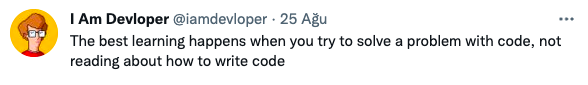
\includegraphics{developer.png}

\hypertarget{instructor-information}{%
\subsection{Instructor Information}\label{instructor-information}}

\textbf{Instructor:} Gül İnan

\textbf{E-mail:}
\href{mailto:inan@itu.edu.tr}{\nolinkurl{inan@itu.edu.tr}}

\textbf{Office:} Room 424 @ Department of Mathematics

\textbf{Office hour:} Send me an e-mail for your queries or for
scheduling an online appointment via Zoom.

\hypertarget{course-information}{%
\subsection{Course Information}\label{course-information}}

\textbf{Course Type:} Elective for undergraduate students.

\textbf{Course Credits:} 3 local credits (6 ECTS credits).

\textbf{Course Prerequisites:} MAT 116/E MIN DD.

\textbf{Course Description:}

Data science is an interdisciplinary and broad field using mathematics,
statistics, and computer science methods and tools to extract
information and insight from data in different forms. This course is an
introductory level data science course on introducing different data
types (structured and unstructured) from different fields arising mostly
from digital technologies or available on the web, and then focusing on
importing, cleaning, reshaping, exploring, and visualizing these data.

\textbf{Computer skills:}

We will be using \texttt{R} programming language with
\texttt{RStudio\ IDE} for data related works. You will be using the
version control system \texttt{Git} along with \texttt{GitHub} to submit
homework assignments and team-based works. Lastly, prior knowledge of
\texttt{HTML}, \texttt{CSS}, and \texttt{JavaScript} brings a big plus
to produce fancy outputs for your works. But it is neither a must nor
focus of this course.

\textbf{Course website:} For each study, you will also receive an
invitation soon to submit your study to the GitHub Classroom of the
following organization:

\url{https://github.com/MAT381E-Fall21}.

\textbf{Class Schedule:} Mondays between 14:30-17:30 p.m. (Local time in
Istanbul).

\textbf{Classroom:} Online via secured ITU Zoom platform.

\textbf{Course Logistics:} Each week, before the class, a Zoom meeting
invitation will be sent you via your ITU email to join the class on
Mondays. Lectures will be automatically recorded and you will have a
chance re-watch the videos after the class on
\url{https://ninova.itu.edu.tr}. Lecture materials (notes, assignments,
grades etc) will be uploaded on \url{https://ninova.itu.edu.tr}.

\textbf{Course Objectives:} This course aims to:

\begin{enumerate}
\def\labelenumi{\arabic{enumi}.}
\tightlist
\item
  Provide basic knowledge required for using data science computational
  tools such as a programming language and its packages associated with
  data science, a dynamic report application, and version control
  system.
\item
  Introduce different types of data from different disciplines arising
  from digital technologies or available on the web.
\item
  To give an ability for accessing, cleaning, reshaping, exploring, and
  visualizing different types of data from different disciplines.
\item
  To give an ability for interpreting data arising from different
  disciplines and making data-driven inferences.
\end{enumerate}

\textbf{Course Tentative Plan}: We will closely follow the weekly
schedule given below. However, weekly class schedules are subject to
change depending on the progress we make as a class.

\begin{longtable}[]{@{}
  >{\centering\arraybackslash}p{(\columnwidth - 4\tabcolsep) * \real{0.23}}
  >{\centering\arraybackslash}p{(\columnwidth - 4\tabcolsep) * \real{0.23}}
  >{\raggedright\arraybackslash}p{(\columnwidth - 4\tabcolsep) * \real{0.55}}@{}}
\toprule
\begin{minipage}[b]{\linewidth}\centering
\textbf{Week}
\end{minipage} & \begin{minipage}[b]{\linewidth}\centering
\textbf{Date}
\end{minipage} & \begin{minipage}[b]{\linewidth}\raggedright
\textbf{Topic}
\end{minipage} \\
\midrule
\endhead
1 & 04/10 & Introduction to data science and computational tools. \\
2 & 11/10 & Tools for data importing, manipulating, and tidying. \\
3 & 18/10 & Basic principles of data visualization. \\
4 & 25/10 & Data visualization tools. \\
5 & 01/11 & Handling with strings and dates in data. \textbf{(HW1
assigned, Project proposal submission)} \\
6 & 08/11 & Scraping data from web. \\
7 & 15/11 & Data extraction from social networking sites. \\
8 & 22/11 & ITU Fall Break. \\
9 & 29/11 & Basic principles of text mining. \textbf{(Project interim
report submission)} \\
10 & 06/12 & Network analysis and visualization. \\
11 & 13/12 & Basic principles of geographic information system. \\
12 & 20/12 & Visualization of spatial and urban data. \textbf{(HW2
assigned)} \\
13 & 27/12 & Basic principles of interactive data visualization. \\
14 & 03/01 & Interactive web-based data visualization tools. \\
15 & 10/01 & Relational databases. \\
16-17 & 17-30/01 & Final exam week. \textbf{(Final report submission,
Project website on GitHub pages, Oral presentation)} \\
\bottomrule
\end{longtable}

\textbf{Student Learning Outcomes:} A student who completed this course
successfully is expected to:

\begin{enumerate}
\def\labelenumi{\arabic{enumi}.}
\tightlist
\item
  Know the recent technologies associated with data science,
\item
  Know basic programming skills with R Programming and get familiar with
  its data science related packages,
\item
  Know how to access data from various sources,
\item
  Know how to clean, reshape, explore, and visualize the data for
  reporting and further analysis.
\item
  Know how to make data-driven inferences,
\item
  Know how to perform reproducible research,
\item
  Know how to present findings both verbally and orally,
\item
  Know how to do collaborative work and effectively work in a team
  environment, and
\item
  Know how to communicate with audience from different disciplines
\end{enumerate}

immediately following the course, and/or a few months after the course.

\textbf{Textbook:} All lecture materials.

\textbf{Course Workload:} 2 homework assignments, a team-based project
(see the details below).

\textbf{Recommended Bibliography:} Students are encouraged to consult
the following sources on their own:

\begin{enumerate}
\def\labelenumi{\arabic{enumi}.}
\item
  Wickham, H. and Grolemund, G. (2016). R for data science: import,
  tidy, transform, visualize, and model data. O'Reilly Media,
  Inc.~{[}Freely available through the book's website
  \url{https://r4ds.had.co.nz/}{]}.
\item
  Bivand, R.S., Pebesma, E.J., Gomez-Rubio, V., and Pebesma, E. J.
  (2013). Applied spatial data analysis with R. New York: Springer. 2nd
  ed.~{[}Electronic resource at ITU Library Services{]}.
\item
  Carson, S. (2020). Interactive web-based data visualization with R,
  plotly, and shiny. CRC Press. {[}Freely available through the book's
  website \url{https://plotly-r.com/}{]}.
\item
  Douglas, A.L. (2015). A user's guide to network analysis in R. Cham:
  Springer International Publishing. 1st ed.~{[}Electronic resource at
  ITU Library Services{]}.
\item
  Silge, J., and Robinson, D. (2017). Text mining with R: A tidy
  approach. O'Reilly Media, Inc.~{[}Freely available through the book's
  website \url{https://www.tidytextmining.com/}{]}.
\item
  Wickham, H. (2016). ggplot2: Elegant graphics for data analysis.
  Springer, 2nd ed.~{[}Electronic resource at ITU Library Services{]}.
\end{enumerate}

\textbf{Off-Campus Access to the ITU Library E-sources:}

Access to library e-sources remotely is possible with a library account.
Users without a library account should apply for the library
registration at \url{https://kutuphane.itu.edu.tr/en/register}. After
setting the web configurations given at
\url{https://kutuphane.itu.edu.tr/en/services}
/web-browser-proxy-settings only once on your computer, you will able to
have an access to ITU Library e-sources.

\textbf{Selected Important Dates:} For the official ITU Fall 2021
academic calendar, please visit:

\url{https://www.sis.itu.edu.tr/TR/ogrenci/akademik-takvim/akademik-takvimler/takvim2022/lisans-akademik-takvimi.php}

Here are some selected important dates in Fall 2021 semester:

October 4, 2021: First day of classes.

October 4-8, 2021: Add-drop week.

October 29, 2021: Republic Day of Turkey (Friday, No classes).

November 22-26, 2021: ITU Fall Break (No classes).

January 1, 2022: New year (Saturday).

January 14, 2022: Last day of classes.

January 17-30, 2022: Final exam week.

I also honor other national and religous holidays. Students, who needs
flexibility on individual-based studies overlapping with these special
days, can inform me.

\hypertarget{course-policies}{%
\subsection{Course Policies}\label{course-policies}}

Please read the information below as a reference for how this class will
be conducted.

\textbf{Grading Policy:}

\begin{itemize}
\item
  Assessment Method Total Contribution to Final Grade:

  \begin{itemize}
  \tightlist
  \item
    2 homework assignments each 10\%,
  \item
    1 team-based project 80\%.
  \item
    Detailed break-down of the team-based project:

    \begin{itemize}
    \tightlist
    \item
      Project proposal 10\%,
    \item
      Project interim written-report 20\%,
    \item
      Project final written-report 20\%,
    \item
      Project website on GitHub pages 5\%,
    \item
      Project final oral presentation 20\%,
    \item
      Peer evaluation 5\%,
    \item
      Statement of personal contribution.
    \end{itemize}
  \end{itemize}
\item
  Exact submission dates for each study above will be announced at well
  in advance.
\item
  Homework assignments are individual-based studies, whereas team-based
  project is the product of team.
\item
  All members of a team will get the same point on \textbf{the project
  proposal, interim report, final report, report posted on GitHub pages,
  and oral presentation}. However, I reserve the right to assign
  different grades to each team member based on peer evaluations (see
  below).
\item
  Each team member should contribute to oral presentation where the
  allocated time is evenly distributed among the team members. If any
  member of the team fails to do oral presentation, that individual will
  receive ``0'' for oral presentation grade.
\item
  The peer evaluation point of a student will be the average of the
  points which his/her team members will assign to him/her.
\item
  If any member for a specific team fails to submit the peer evaluation
  form, all members of that team will receive ``0'' for peer evaluation
  grade.
\item
  \textbf{For detailed information on project design guideline and
  related documents, please see the relevant document on Ninova.}
\item
  \textbf{Every study mentioned above should be submitted by each
  student via GitHub Classroom of MAT381E-Fall21 organization.}
\end{itemize}

\textbf{Late Submission Policy:} Students are expected to do homework
assignments by themselves. Neither homework assignments nor team-based
works will be accepted after deadline. There are \textbf{NO} make-ups
for missed homework and team-based works. The students who have Covid-19
medical report during the submission periods can ask for extension only.

\textbf{Final Exam Attendance Policy:} None.

\textbf{Make-Up Exam Policy:} Not applicable this semester.

\textbf{Class Attendance Policy:}

The students must attend at least 70\% of classes and are deemed
responsible to manage his/her absences.

\textbf{Participation Policy:}

The students are expected to ask and answer questions, participate in
in-class activities, and show their interest and engagement in the
class.

\textbf{E-mail Policy:}

Please:

\begin{enumerate}
\def\labelenumi{\arabic{enumi}.}
\tightlist
\item
  Use a proper descriptive subject line (which may consist of the course
  number MAT381E followed by a short phrase summarizing the subject of
  your e-mail).
\item
  Start off your e-mail with a proper greeting, introduce yourself (give
  your name), then state your problem as short as possible.
\item
  Finally, use a proper closing and then finish your e-mail with your
  first name and so on.
\end{enumerate}

Feel free to send me e-mails. But be sure you that give me enough time
to get back to you. In the past, I have had pretty much tolerance for
e-mail messages sent after business hours and at weekends. But, now, due
to pandemic, I should say that I may not appreciate these e-mails
anymore. Lastly, e-mails asking for grade grubbing at the end of the
semester are not welcomed.

\textbf{Equity, Diversity, and Inclusion:}

In this class, I am committed to cultural and individual differences and
diversity as including, but not limited to, age, disability, ethnicity,
gender, gender identity, language, national origin, race, religion,
culture, and socioeconomic status and I acknowledge the value of
differences.

\textbf{Academic Honesty Policy:}

At every stage of the academic life, every ITU student is responsible
for obeying the academic honesty policy of ITU stated below:

\url{https://odek.itu.edu.tr/en/code-of-honor/ethics-in-university-life}.

\textbf{Student with Special Needs:}

If you are a student with special needs, let me know that how we can
adjust the course environment and materials in accordance with your
needs. Furthermore, you are also invited to contact the office of
students with special needs at:

\url{http://engelsiz.itu.edu.tr/}.

\textbf{ITU Distance Education Policy:}

Sharing the lecture recordings or its piece with third parties is
strictly forbidden. Furthermore, the recordings are subject to
investigation by the authorities as needed. For that reason, be sure
that you behave (both orally and verbally) responsibly in this virtual
class. Please visit:

\url{https://online.itu.edu.tr/},

for more information on distance education regulations at ITU.

\end{document}
